\section{Results}

\subsection{Setup}

As input to the closure test, a single replica was drawn randomly from
a previous NNPDF fit to experimental data. We refer to this as the underlying
law and the corresponding observables the true observable values. An example
of the gluon input is provided in Fig.~\ref{fig:InputGluonPDF}.

\begin{figure}
    \centering
    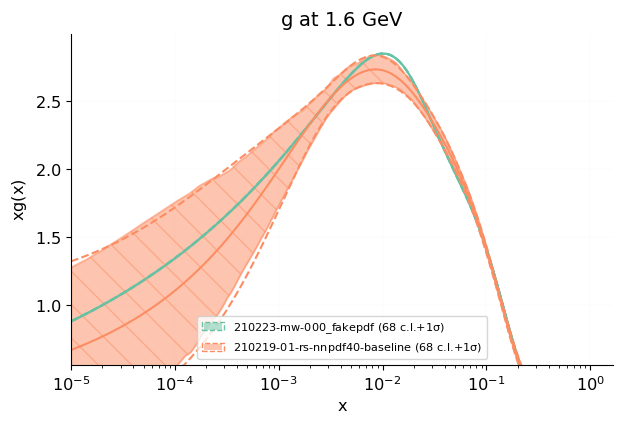
\includegraphics[width=0.6 \textwidth]{plot_pdfs_g.png}
    \caption{The green line is the input underlying law for the gluon PDF,
    which is sampled from the ensemble from a fit to data. The 68\% confidence
    interval is plotted for those replicas as the orange band.}
    \label{fig:InputGluonPDF}
\end{figure}

We then sampled 30 different sets of experimental central values (or L1 data),
by drawing
shifts from the experimental covariance matrix as described in
Eq.~\ref{eq:levelonedata}. Each set of experimental central values was then
fitted following the usual NNPDF methodology, fitting pseudo-data replicas.

The methodology and hyperparameters we tested here was identical to that used
to produce the upcoming NNPDF4.0 PDF sets, full details of how those hyperparameters
were chosen and the impact on PDFs from a phenomonological standpoint will be
discussed in \cite{NNPDF40}. % add in preparation citation.
The results presented here are part of a series of validation checks we have performed
on the new NNPDF4.0 methodology, alongside the "future test" presented in
\cite{Cruz_Martinez_2021}.

The PDFs are fitted to a subset of the full NNPDF4.0 dataset. For convenience,
we chose to fit the PDFs on a variant of the NNPDF3.1 dataset used in
\cite{Ball_2018}, which is described in detail in a study of the determination
of the strange PDF \cite{Faura_2020}. The datasets used in the calculation of
statistical estimators are the new datasets which will be included in NNPDF4.0,
and are summarised in Tab.~\ref{tab:summarise_new_data}, but not discussed in detail.

\begin{table}[h!]
    \begin{center}
    \resizebox{0.6\textwidth}{!}{\begin{tabular}{llll}
        \toprule
        {} & Training fraction & C-factors & Other fields \\
        Dataset                                &                   &           &              \\
        \midrule
        ATLASPHT12                             &                 - &       QCD &            - \\
        ATLASPHT15                             &                 - &       QCD &            - \\
        ATLAS\_SINGLETOP\_TCH\_R\_7TEV             &                 - &       QCD &            - \\
        ATLAS\_SINGLETOP\_TCH\_DIFF\_7TEV\_T\_PT     &                 - &       QCD &            - \\
        ATLAS\_SINGLETOP\_TCH\_DIFF\_7TEV\_T\_RAP    &                 - &       QCD &            - \\
        ATLAS\_SINGLETOP\_TCH\_DIFF\_7TEV\_TBAR\_PT  &                 - &       QCD &            - \\
        ATLAS\_SINGLETOP\_TCH\_DIFF\_7TEV\_TBAR\_RAP &                 - &       QCD &            - \\
        ATLAS\_SINGLETOP\_TCH\_R\_8TEV             &                 - &       QCD &            - \\
        ATLAS\_SINGLETOP\_TCH\_DIFF\_8TEV\_T\_PT     &                 - &       QCD &            - \\
        ATLAS\_SINGLETOP\_TCH\_DIFF\_8TEV\_T\_RAP    &                 - &       QCD &            - \\
        ATLAS\_SINGLETOP\_TCH\_DIFF\_8TEV\_TBAR\_PT  &                 - &       QCD &            - \\
        ATLAS\_SINGLETOP\_TCH\_DIFF\_8TEV\_TBAR\_RAP &                 - &       QCD &            - \\
        ATLAS\_SINGLETOP\_TCH\_R\_13TEV            &                 - &       QCD &            - \\
        ATLAS\_2JET\_7TEV\_R06                    &                 - &  QCD, EWK &            - \\
        ATLAS\_2JET\_7TEV\_R04                    &                 - &  QCD, EWK &            - \\
        ATLAS\_WP\_JET\_8TEV\_PT                   &                 - &       QCD &            - \\
        ATLAS\_WM\_JET\_8TEV\_PT                   &                 - &       QCD &            - \\
        ATLAS\_WP\_JET\_8TEV\_PTJ                  &                 - &       QCD &            - \\
        CMS\_SINGLETOP\_TCH\_TOT\_7TEV             &                 - &       QCD &            - \\
        CMS\_SINGLETOP\_TCH\_R\_8TEV               &                 - &       QCD &            - \\
        CMS\_SINGLETOP\_TCH\_R\_13TEV              &                 - &       QCD &            - \\
        CMS\_2JET\_7TEV                          &                 - &  QCD, EWK &            - \\
        CMS\_2JET\_3D\_8TEV                       &                 - &  QCD, EWK &            - \\
        \bottomrule
        \end{tabular}}
\end{center}
    \caption{Summary of the new processes, out of sample data used to compute the statistical estimators.}
    \label{tab:summarise_new_data}
\end{table}

The choice of fitted datasets is
considered unimportant, one could consider splitting the data into training
and test in a way which considered kinematic coverage rather than this
naive chronological splitting. Alternatively, since the data is generated from
the theory predictions produced by the input underlying law, one could even
produce completely artificial data using a different set of FK tables. From a
practical standpoint, using the NNPDF3.1 dataset and validating on the newly
included
datasets in 4.0 allowed us to validate the PDF uncertainities on data outside
of the kinematic coverage of data included in the fit. In appendix {\bf TODO}
we calculate the closure estimators on fitted data, although as discussed the
meaning of these estimators is less clear.

\subsection{Bias-variance ratio $\biasvarratio$}

We calculated $\biasvarratio$ on the test data, shown in
Tab.~\ref{tab:summarise_new_data}. An
uncertainty on $\biasvarratio$ by performing a bootstrap sample
\cite{efron1994introduction},
where we randomly sample from both fits and replicas and re-calculate
$\biasvarratio$, the value and error presented in the table is then the mean
and standard deviation across bootstrap samples. We checked that the distribution
of the estimator across bootstrap samples is indeed Gaussian.
% TODO?
% , and show it
% explicitly
% in Appendix {\bf TODO}.

\begin{table}
    \begin{center}
        \begin{tabular}{lr}
            \toprule
            {} &  $\biasvarratio$ \\
            experiment &                      \\
            \midrule
            ATLAS       &                 $1.04 \pm 0.04$  \\
            CMS         &                 $1.04 \pm 0.06$ \\
            LHCb       &                 $0.82 \pm 0.06$ \\
            Total       &                 $ 1.03 \pm 0.05$ \\
            \bottomrule
        \end{tabular}
    \end{center}
    \caption{
        The bias-variance ratio, $\biasvarratio$, for unfitted data, summarised in
        Tab.~\ref{tab:summarise_new_data}. Generally $\biasvarratio$ is within
        $1\sigma$ of 1, except for LHCb where there is a $3\sigma$ deviation.
        There are, however fewer datapoints included in LHCb and so this could be
        a statistical fluctuation. Furthermore, if this result were to hold as
        more data was added in these kinematic regions, it suggests that the
        uncertainties are slightly overestimated (on the level of 20\%) which is
        is at worst a bit conservative, and preferable to underestimated
        uncertainities. Finally, across all data we find $\biasvarratio$ to
        be compatible with 1.
    }
    \label{tab:biasvarratio}
\end{table}

One can also compare qualitatively the distribution of bias across fits, to the
distribution of the difference between replica predictions and expectation
values of predictions (in units of the covariance) across different fits
and replicas. The square root ratio of the mean of these two distributions
is precisely $\biasvarratio$.

\begin{figure}
    \centering
    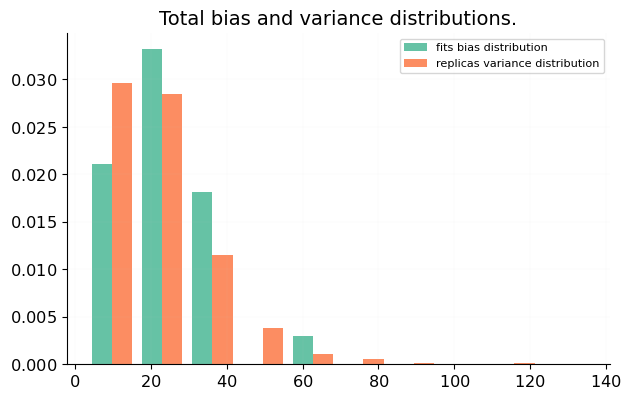
\includegraphics[width=0.6 \textwidth]{plot_bias_variance_distributions_total.png}
    \caption{The green histogram is the distribution of the total bias across fits,
    the orange histogram is the distribution of the difference between the
    replica and central predictions squared, in units of the covariance
    across all fits and replicas. This gives a qualitative picture of the full
    distribution, in Tab.~\ref{tab:biasvarratio} we compare the square root of the
    mean of each distribution.}
\end{figure}

\subsection{Comparison to $\xi_{1\sigma}$}

As discussed in Sec.~\ref{sec:QuantileStatistics}, one can define an analogous
estimator in data space, based upon $\xi_{n\sigma}$, which was defined on a grid
of points in $x$ and $Q^2$ in PDF space in \cite{nnpdf30}. There is not
a one-to-one correspondence
between this and $\biasvarratio$, but a loose approximation using
Eq.~\ref{eq:expectedxi}. In Tab.~{\bf TODO} we compare the estimated
$\xi_{1\sigma}$ from
subsituting $\biasvarratio$ into Eq.~\ref{eq:expectedxi} and to the
measured value.

\begin{table}
    \begin{center}
        \begin{tabular}{lrr}
            \toprule
            {} &  $\xi_{1\sigma}$ &  est. from $\biasvarratio$ \\
            experiment &  &                \\
            \midrule
            ATLAS       &  $0.70 \pm 0.02$ &  $0.66 \pm 0.02$ \\
            CMS         &  $0.68 \pm 0.02$ &  $0.67 \pm 0.03$ \\
            LHCb        &  $0.69 \pm 0.04$ &  $0.78 \pm 0.04$ \\
            Total       &  $0.69 \pm 0.02$ &  $0.67 \pm 0.02$ \\
            \bottomrule
        \end{tabular}
    \end{center}
    \caption{
        Comparing the measured value of $\xi_1\sigma$ and the estimated
        value from $\biasvarratio$. The two columns are consistent, which
        suggests the approximation that the ratio of uncertainties is
        approximately the same across all data is not completely invalidated.
        The largest discrepancy is with LHCb, which in Tab.~\ref{tab:biasvarratio}
        was shown to possibly have slightly overestimated uncertainties. Here we
        see that the measure $\xi_1\sigma$ is completely consistent with 0.68,
        which possibly suggests that the $\biasvarratio$ is dominated by some
        eigenvectors of the uncertainty having. The breakdown of $\xi_1\sigma$
        for each eigenvector of LHCb can be seen in
        Fig.~\ref{fig:xibreakdownlhcb}, which further supports this.
    }
    \label{tab:xicomparison}
\end{table}

Despite the assumptions entering each of the two estimators differing, we see
good agreement between the $\xi_{1\sigma}$ estimated from $\biasvarratio$
and that measured directly. We find this result reassuring, since it indicates
not only that the total uncertainty averaged across all data is faithful, but
also that the uncertainty on each data point seems faithful. If the results
differed it would indicate some kind of imbalance, where some components
of the uncertainty are correctly represented by the replicas but other directions
are not.

\begin{figure}
    \centering
    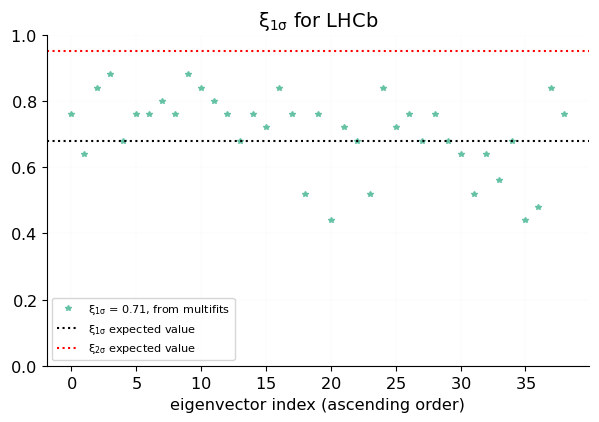
\includegraphics[width=0.6 \textwidth]{lhcbxi_data.png}
    \caption{$\xi_1\sigma$ for each eigenvector of the experimental
    covaraince matrix. We see that the first few eigenvectors have over
    estimated uncertainty, but the latter are more evenly distributed
    around 0.68. The suggested overestimated uncertainty by $\biasvarratio$
    is likely dominated by the first few eigenvectors.}
    \label{fig:xibreakdownlhcb}
\end{figure}
